
\documentclass[12pt,a4paper]{article}
\usepackage{fontspec}
\setmainfont{DejaVu Sans}
\usepackage[a4paper,margin=2.2cm]{geometry}
\usepackage{graphicx}
\usepackage{float}
\usepackage{booktabs}
\usepackage{longtable}
\usepackage{array}
\usepackage{hyperref}
\usepackage{amsmath}
\usepackage{enumitem}
\hypersetup{colorlinks=true, linkcolor=blue, urlcolor=blue}
\setlength{\parindent}{0pt}
\setlength{\parskip}{6pt}
\renewcommand{\arraystretch}{1.25}

\begin{document}

\begin{center}
    {\Large\textbf{BÁO CÁO THỰC HÀNH 01}}\\[4pt]
    {\large\textbf{OpenCV Basic - Xử lý ảnh cơ bản}}\\[8pt]
    \textbf{Tên nhóm:} \underline{\hspace{7cm}}\\
    \textbf{MSHV1:} \underline{\hspace{4cm}} \quad
    \textbf{MSHV2:} \underline{\hspace{4cm}}
\end{center}

\section{Mục tiêu}

Bài thực hành xây dựng một Jupyter Notebook xử lý ảnh cơ bản. Các nội dung gồm đọc và hiển thị ảnh, scale, xoay ảnh, biến đổi màu sắc, độ sáng và độ tương phản. Notebook được chia lại theo yêu cầu: mỗi mục lớn có 3 code cell chính gồm cell thủ công, cell dùng thư viện và cell so sánh thời gian hoặc bộ nhớ.

\section{Cấu trúc bài nộp}

Gói nộp được tổ chức như sau:

\begin{itemize}[leftmargin=1.2cm]
    \item \texttt{source/}: chứa notebook, ảnh dự phòng, \texttt{requirements.txt}, \texttt{environment.yml}, \texttt{README.md} và thư mục kết quả.
    \item \texttt{doc/}: chứa báo cáo PDF, nguồn LaTeX và hình ảnh minh chứng.
    \item File nén cuối cùng theo mẫu \texttt{TenNhom\_MSHV1\_MSHV2\_th01.zip}.
\end{itemize}

\section{Ảnh đầu vào}

Notebook có cell tải ảnh từ Internet bằng lệnh:

\begin{quote}
\small
\texttt{wget -q -O data/Lenna.jpg}\\
\texttt{http://www.ess.ic.kanagawa-it.ac.jp/std\_img/colorimage/Lenna.jpg}
\end{quote}

Nếu môi trường không có Internet, notebook tự tạo ảnh dự phòng để toàn bộ cell vẫn chạy được. Cách này giúp bài nộp không phụ thuộc tuyệt đối vào mạng trong lúc chấm.

\section{Thư viện sử dụng}

\begin{longtable}{p{0.24\textwidth}p{0.66\textwidth}}
\toprule
\textbf{Thư viện} & \textbf{Vai trò} \\
\midrule
\texttt{NumPy} & Tự cài đặt các phép biến đổi trên ma trận pixel. \\
\texttt{OpenCV} & Đọc ảnh, ghi ảnh và dùng hàm thư viện để đối chiếu. \\
\texttt{Matplotlib} & Hiển thị ảnh trong notebook. \\
\texttt{time} & Đo thời gian chạy. \\
\texttt{tracemalloc} & Đo bộ nhớ Python cấp phát ở mức xấp xỉ. \\
\bottomrule
\end{longtable}

\section{Tổ chức notebook}

Mỗi mục xử lý chính được chia theo đúng 3 cell:

\begin{enumerate}[leftmargin=1.2cm]
    \item \textbf{CELL THỦ CÔNG}: tự cài đặt bằng NumPy và thao tác pixel.
    \item \textbf{CELL TỰ ĐỘNG / THƯ VIỆN}: dùng hàm OpenCV tương ứng.
    \item \textbf{CELL SO SÁNH}: hiển thị ảnh, tính MSE, đo thời gian và bộ nhớ.
\end{enumerate}

\section{Minh chứng chức năng}

\subsection{Đọc và hiển thị ảnh}

Phần thủ công tự chuyển BGR sang RGB bằng thao tác slicing. Phần thư viện dùng \texttt{cv2.cvtColor}. Vì OpenCV đọc ảnh theo thứ tự BGR còn Matplotlib hiển thị theo RGB, bước chuyển kênh là bắt buộc.

\begin{figure}[H]
    \centering
    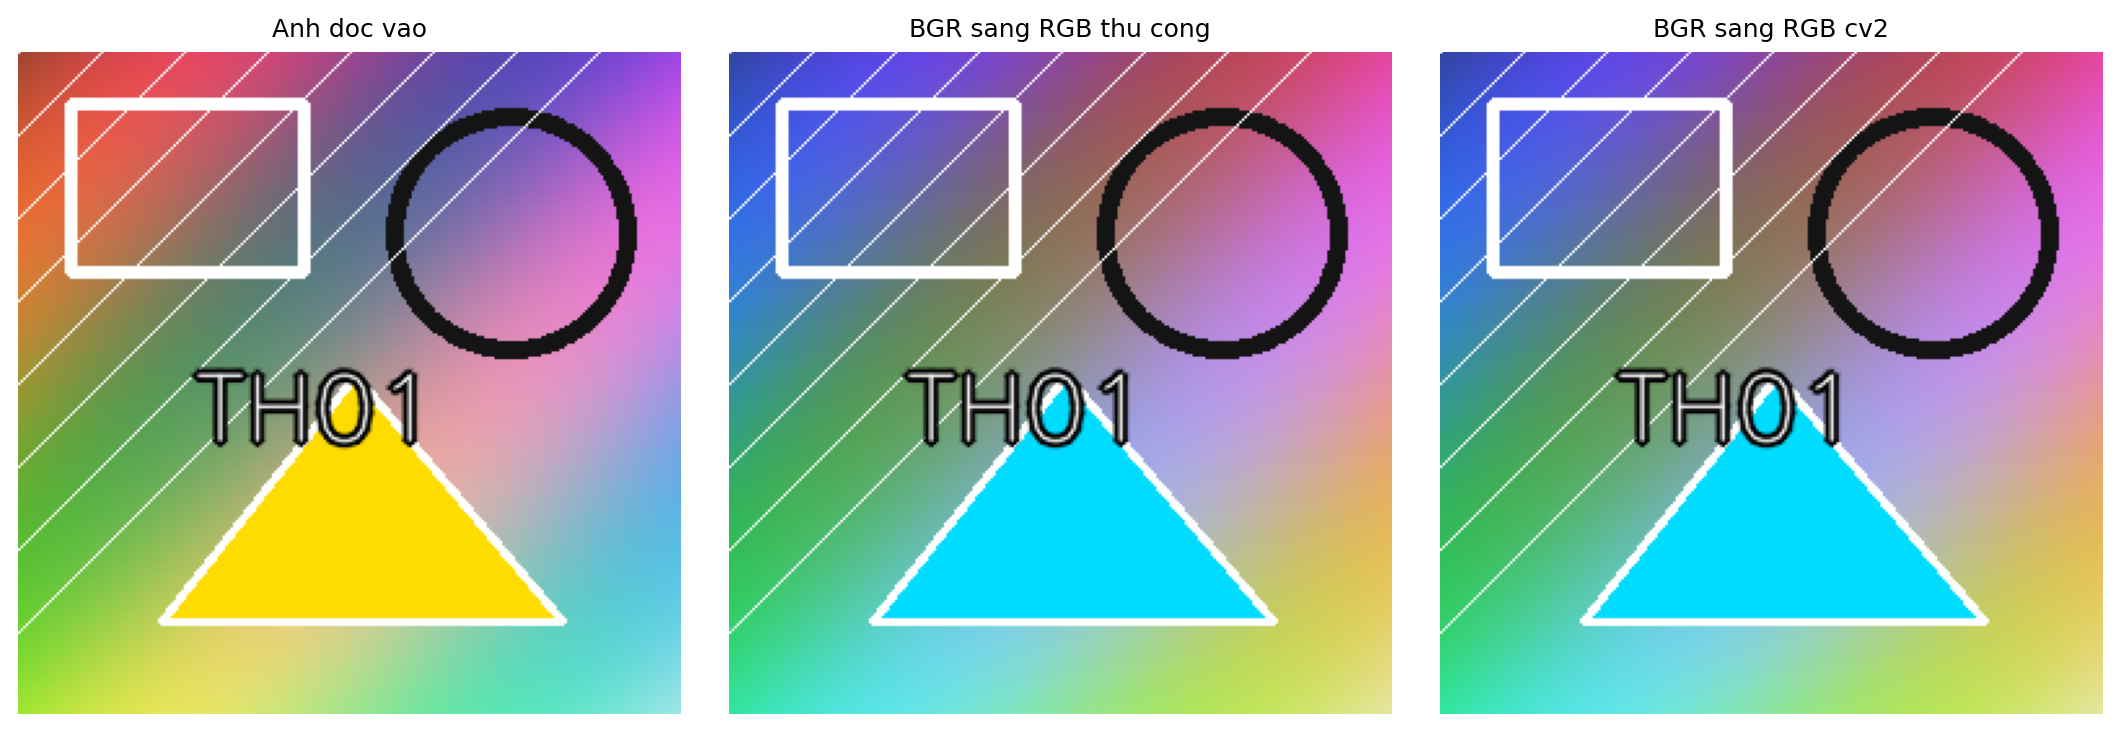
\includegraphics[width=0.95\textwidth]{figures/01_open_show.png}
    \caption{Minh chứng đọc ảnh và chuyển BGR sang RGB.}
\end{figure}

\subsection{Scale ảnh}

Phần thủ công cài đặt nội suy bilinear. Với mỗi pixel đầu ra, thuật toán ánh xạ về vị trí thực trên ảnh nguồn, lấy bốn pixel lân cận và nội suy theo hai chiều. Phần thư viện dùng \texttt{cv2.resize} với \texttt{INTER\_LINEAR}.

\begin{figure}[H]
    \centering
    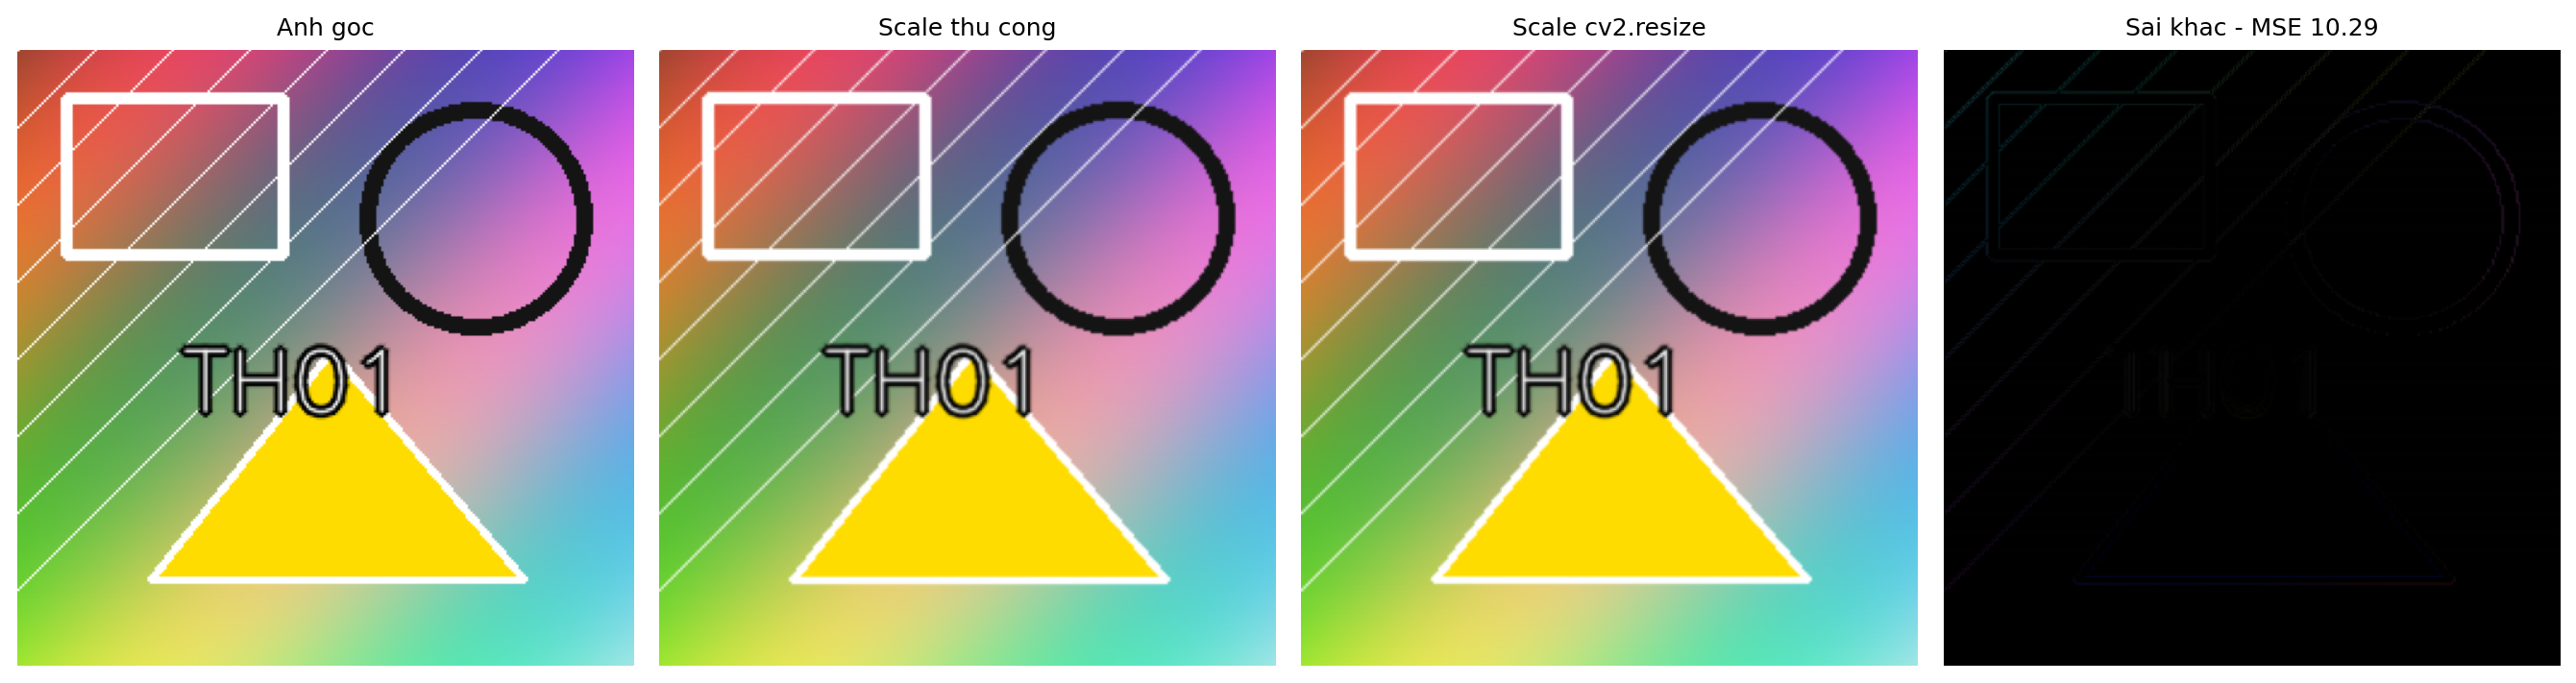
\includegraphics[width=\textwidth]{figures/02_scale.png}
    \caption{So sánh scale thủ công và scale bằng OpenCV.}
\end{figure}

\subsection{Xoay ảnh}

Phần thủ công dùng ánh xạ ngược quanh tâm ảnh. Với mỗi pixel đầu ra, thuật toán tính ngược tọa độ nguồn rồi lấy pixel gần nhất. Phần thư viện dùng \texttt{cv2.getRotationMatrix2D} và \texttt{cv2.warpAffine}.

\begin{figure}[H]
    \centering
    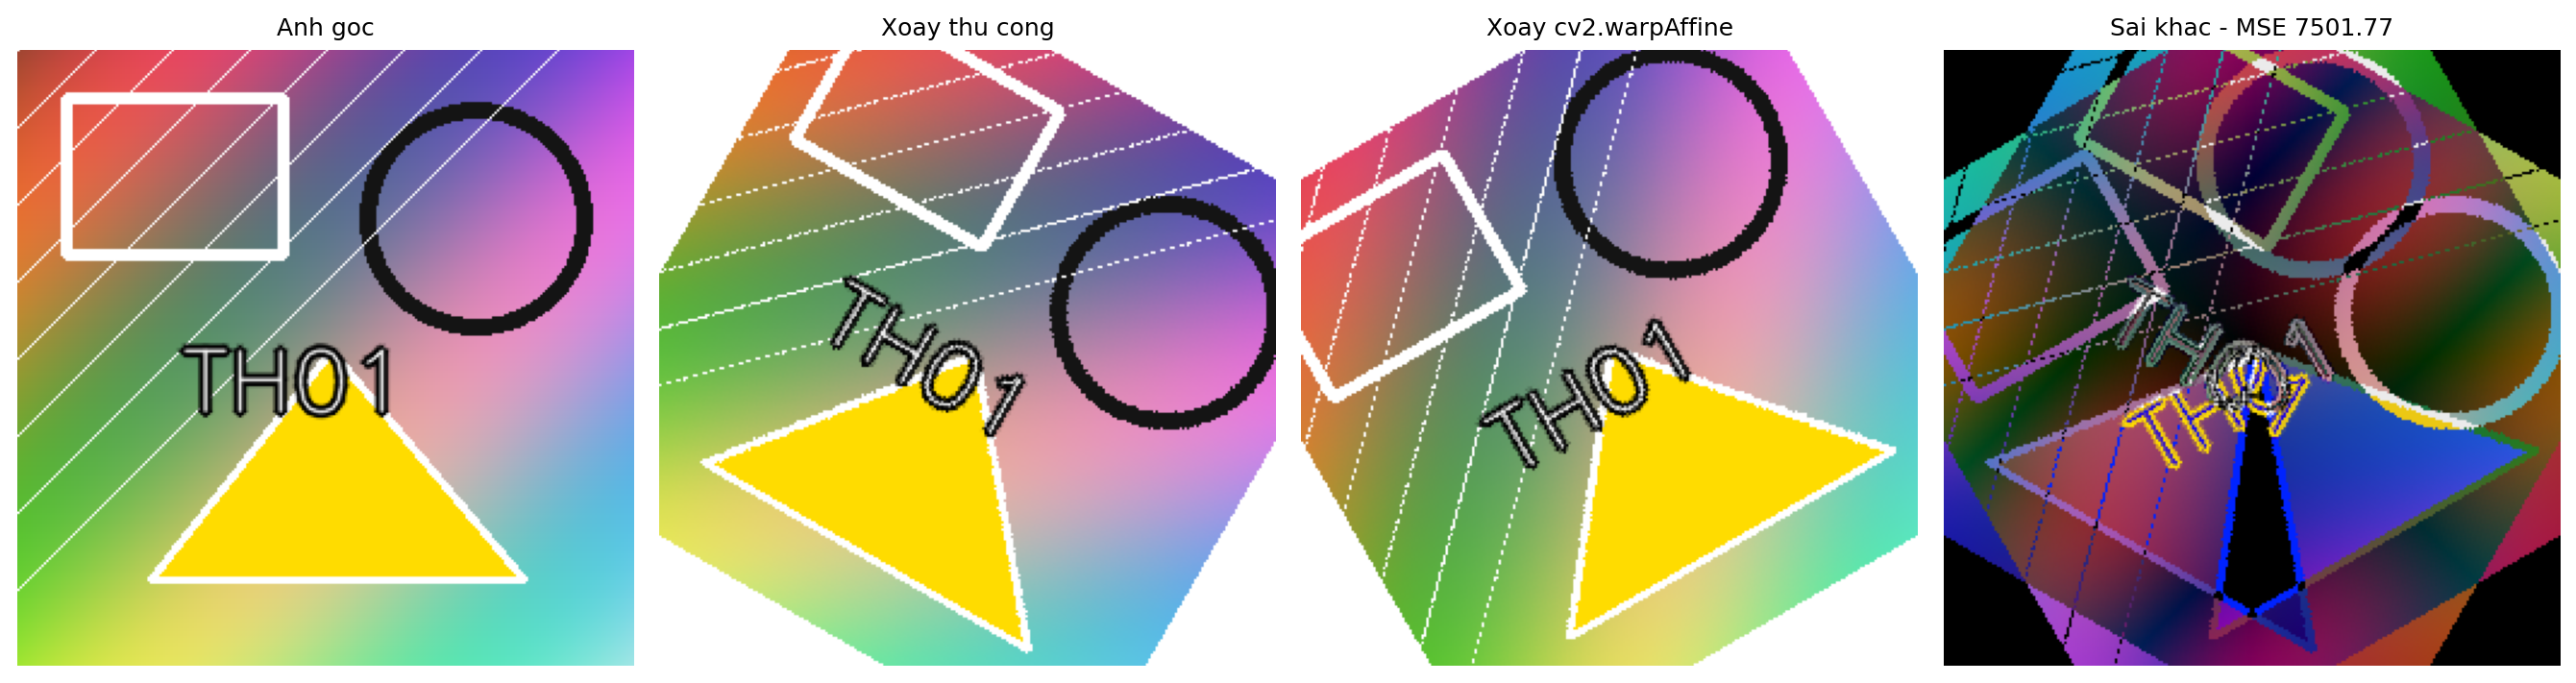
\includegraphics[width=\textwidth]{figures/03_rotate.png}
    \caption{So sánh xoay ảnh thủ công và xoay bằng OpenCV.}
\end{figure}

\subsection{Biến đổi màu sắc}

Chuyển xám thủ công dùng công thức:

\[
Y = 0.114B + 0.587G + 0.299R
\]

Ảnh âm bản dùng công thức:

\[
I' = 255 - I
\]

\begin{figure}[H]
    \centering
    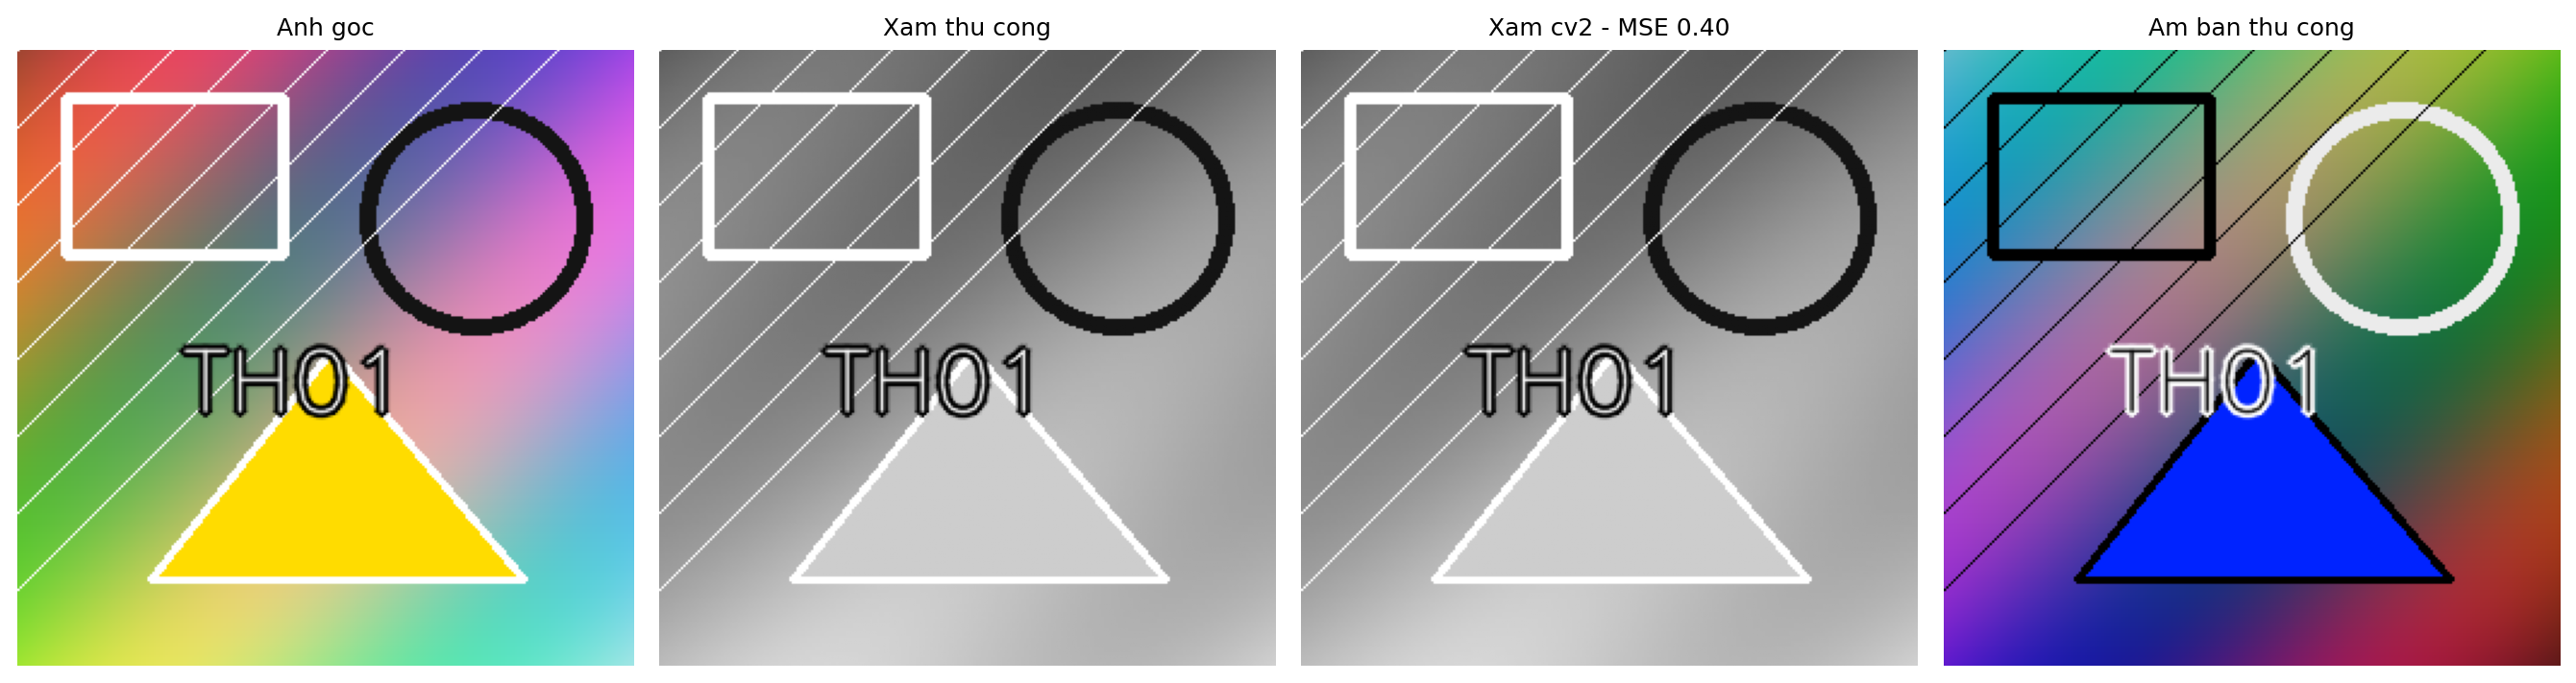
\includegraphics[width=\textwidth]{figures/04_color.png}
    \caption{Minh chứng chuyển xám và tạo ảnh âm bản.}
\end{figure}

\subsection{Độ sáng và độ tương phản}

Phép biến đổi thủ công dùng công thức:

\[
I' = \alpha I + \beta
\]

Trong đó \(\alpha\) điều chỉnh tương phản và \(\beta\) điều chỉnh độ sáng. Kết quả được chặn trong khoảng 0 đến 255. Phần thư viện dùng \texttt{cv2.convertScaleAbs}.

\begin{figure}[H]
    \centering
    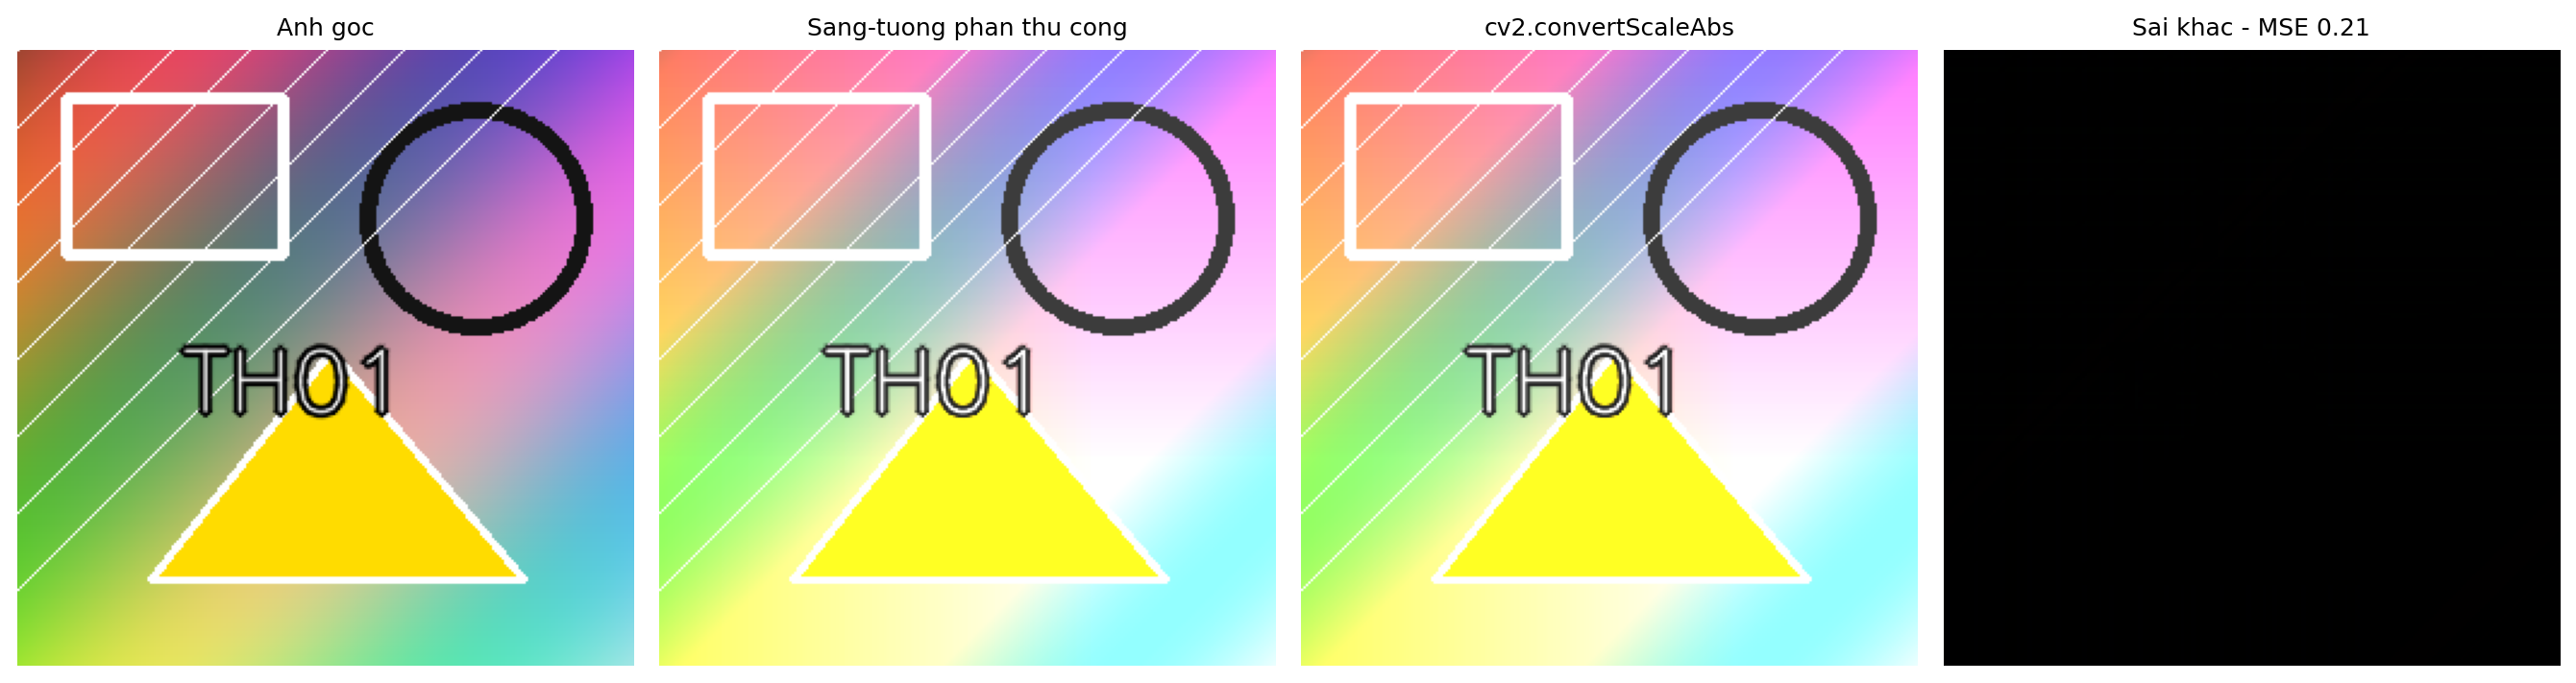
\includegraphics[width=\textwidth]{figures/05_brightness_contrast.png}
    \caption{So sánh chỉnh sáng và tương phản thủ công với OpenCV.}
\end{figure}

\section{So sánh và phân tích}

Các kết quả thủ công và thư viện có thể không trùng tuyệt đối. Nguyên nhân thường nằm ở quy ước làm tròn, vị trí tâm pixel, cách xử lý biên và chi tiết nội suy trong OpenCV. Hàm thư viện thường nhanh hơn vì được tối ưu ở mức C/C++, trong khi cài đặt thủ công dùng vòng lặp Python nên chậm hơn nhưng giúp hiểu rõ bản chất thuật toán.

Bộ nhớ đo bằng \texttt{tracemalloc} chỉ phản ánh bộ nhớ Python cấp phát. Bộ nhớ nội bộ của OpenCV ở tầng C/C++ có thể không được ghi nhận đầy đủ, vì vậy số liệu memory nên dùng để tham khảo tương đối.

\section{Bảng tự đánh giá}

\begin{longtable}{p{0.46\textwidth}p{0.18\textwidth}p{0.26\textwidth}}
\toprule
\textbf{Yêu cầu} & \textbf{Trạng thái} & \textbf{Ghi chú} \\
\midrule
Đọc và hiển thị ảnh & Hoàn thành & Có cell wget, open và show. \\
Scale thay đổi kích thước & Hoàn thành & Có thủ công, thư viện và so sánh. \\
Xoay ảnh & Hoàn thành & Có ánh xạ ngược và \texttt{warpAffine}. \\
Biến đổi màu sắc & Hoàn thành & Có grayscale và âm bản. \\
Độ sáng, độ tương phản & Hoàn thành & Có công thức thủ công và OpenCV. \\
Cell thủ công & Hoàn thành & Mỗi mục lớn có cell riêng. \\
Cell tự động / thư viện & Hoàn thành & Dùng hàm OpenCV tương ứng. \\
Cell so sánh thời gian hoặc memory & Hoàn thành & Có thời gian, memory xấp xỉ, MSE và hình ảnh. \\
Có file đặc tả thư viện & Hoàn thành & Có \texttt{requirements.txt} và \texttt{environment.yml}. \\
Báo cáo riêng, không đưa mã nguồn & Hoàn thành & Báo cáo dùng mô tả, công thức, bảng và hình minh chứng. \\
\bottomrule
\end{longtable}

\section{Phân công đóng góp}

\begin{longtable}{p{0.22\textwidth}p{0.48\textwidth}p{0.20\textwidth}}
\toprule
\textbf{Thành viên} & \textbf{Công việc} & \textbf{Tỉ lệ} \\
\midrule
MSHV1 - Họ tên: \underline{\hspace{3cm}} & Chuẩn bị notebook, phần open/show, scale, xoay và kiểm thử. & 50\% \\
MSHV2 - Họ tên: \underline{\hspace{3cm}} & Phần màu sắc, sáng/tương phản, báo cáo và tổng hợp hình minh chứng. & 50\% \\
\bottomrule
\end{longtable}

\section{Kết luận}

Notebook đã được tổ chức theo đúng hướng yêu cầu: mỗi mục có cell thủ công, cell thư viện và cell so sánh. Cách trình bày này giúp việc chấm bài rõ ràng hơn, đồng thời làm nổi bật sự khác biệt giữa tự cài đặt thuật toán và dùng hàm tối ưu sẵn có.

\end{document}
